\documentclass[10pt]{article}
\usepackage{tikz}
\usetikzlibrary{shapes.misc}
\usepackage[margin=0cm]{geometry}
\pagestyle{empty}
\tikzstyle{every node}=[cross out, draw, red]

\begin{document}

\vspace*{\fill}
\begin{center}
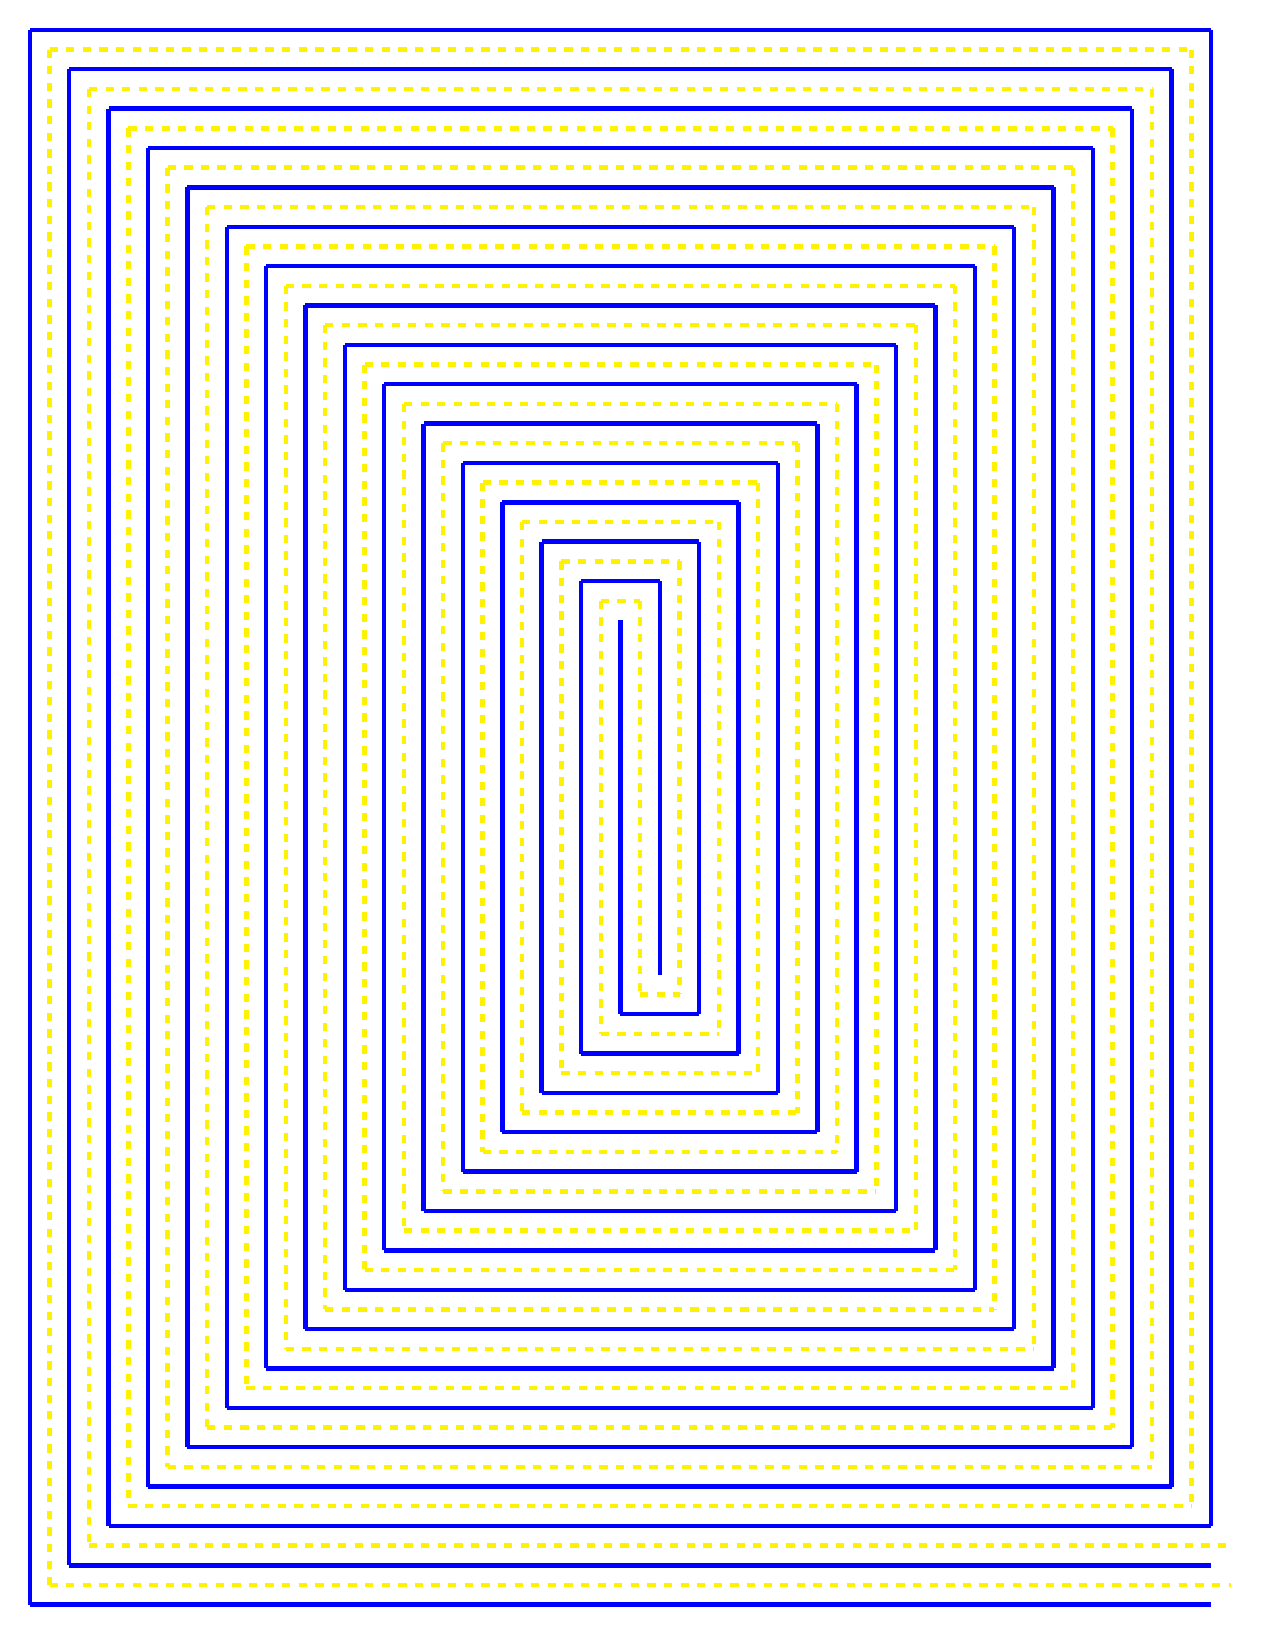
\begin{tikzpicture}[x=0.5cm, y=-0.5cm, ultra thick, blue]
% Walls
    \draw (0,0) -- (30,0);
    \draw (1,1) -- (29,1);
    \draw (2,2) -- (28,2);
    \draw (3,3) -- (27,3);
    \draw (4,4) -- (26,4);
    \draw (5,5) -- (25,5);
    \draw (6,6) -- (24,6);
    \draw (7,7) -- (23,7);
    \draw (8,8) -- (22,8);
    \draw (9,9) -- (21,9);
    \draw (10,10) -- (20,10);
    \draw (11,11) -- (19,11);
    \draw (12,12) -- (18,12);
    \draw (13,13) -- (17,13);
    \draw (14,14) -- (16,14);
    \draw (15,25) -- (17,25);
    \draw (14,26) -- (18,26);
    \draw (13,27) -- (19,27);
    \draw (12,28) -- (20,28);
    \draw (11,29) -- (21,29);
    \draw (10,30) -- (22,30);
    \draw (9,31) -- (23,31);
    \draw (8,32) -- (24,32);
    \draw (7,33) -- (25,33);
    \draw (6,34) -- (26,34);
    \draw (5,35) -- (27,35);
    \draw (4,36) -- (28,36);
    \draw (3,37) -- (29,37);
    \draw (2,38) -- (30,38);
    \draw (1,39) -- (30,39);
    \draw (0,40) -- (30,40);
    \draw (0,0) -- (0,40);
    \draw (1,1) -- (1,39);
    \draw (2,2) -- (2,38);
    \draw (3,3) -- (3,37);
    \draw (4,4) -- (4,36);
    \draw (5,5) -- (5,35);
    \draw (6,6) -- (6,34);
    \draw (7,7) -- (7,33);
    \draw (8,8) -- (8,32);
    \draw (9,9) -- (9,31);
    \draw (10,10) -- (10,30);
    \draw (11,11) -- (11,29);
    \draw (12,12) -- (12,28);
    \draw (13,13) -- (13,27);
    \draw (14,14) -- (14,26);
    \draw (15,15) -- (15,25);
    \draw (16,14) -- (16,24);
    \draw (17,13) -- (17,25);
    \draw (18,12) -- (18,26);
    \draw (19,11) -- (19,27);
    \draw (20,10) -- (20,28);
    \draw (21,9) -- (21,29);
    \draw (22,8) -- (22,30);
    \draw (23,7) -- (23,31);
    \draw (24,6) -- (24,32);
    \draw (25,5) -- (25,33);
    \draw (26,4) -- (26,34);
    \draw (27,3) -- (27,35);
    \draw (28,2) -- (28,36);
    \draw (29,1) -- (29,37);
    \draw (30,0) -- (30,38);
% Pillars
% Inner points in accessible cul-de-sacs
% Entry-exit paths without intersections
    \draw[dashed, yellow] (0.5,0.5) -- (29.5,0.5);
    \draw[dashed, yellow] (1.5,1.5) -- (28.5,1.5);
    \draw[dashed, yellow] (2.5,2.5) -- (27.5,2.5);
    \draw[dashed, yellow] (3.5,3.5) -- (26.5,3.5);
    \draw[dashed, yellow] (4.5,4.5) -- (25.5,4.5);
    \draw[dashed, yellow] (5.5,5.5) -- (24.5,5.5);
    \draw[dashed, yellow] (6.5,6.5) -- (23.5,6.5);
    \draw[dashed, yellow] (7.5,7.5) -- (22.5,7.5);
    \draw[dashed, yellow] (8.5,8.5) -- (21.5,8.5);
    \draw[dashed, yellow] (9.5,9.5) -- (20.5,9.5);
    \draw[dashed, yellow] (10.5,10.5) -- (19.5,10.5);
    \draw[dashed, yellow] (11.5,11.5) -- (18.5,11.5);
    \draw[dashed, yellow] (12.5,12.5) -- (17.5,12.5);
    \draw[dashed, yellow] (13.5,13.5) -- (16.5,13.5);
    \draw[dashed, yellow] (14.5,14.5) -- (15.5,14.5);
    \draw[dashed, yellow] (15.5,24.5) -- (16.5,24.5);
    \draw[dashed, yellow] (14.5,25.5) -- (17.5,25.5);
    \draw[dashed, yellow] (13.5,26.5) -- (18.5,26.5);
    \draw[dashed, yellow] (12.5,27.5) -- (19.5,27.5);
    \draw[dashed, yellow] (11.5,28.5) -- (20.5,28.5);
    \draw[dashed, yellow] (10.5,29.5) -- (21.5,29.5);
    \draw[dashed, yellow] (9.5,30.5) -- (22.5,30.5);
    \draw[dashed, yellow] (8.5,31.5) -- (23.5,31.5);
    \draw[dashed, yellow] (7.5,32.5) -- (24.5,32.5);
    \draw[dashed, yellow] (6.5,33.5) -- (25.5,33.5);
    \draw[dashed, yellow] (5.5,34.5) -- (26.5,34.5);
    \draw[dashed, yellow] (4.5,35.5) -- (27.5,35.5);
    \draw[dashed, yellow] (3.5,36.5) -- (28.5,36.5);
    \draw[dashed, yellow] (2.5,37.5) -- (29.5,37.5);
    \draw[dashed, yellow] (1.5,38.5) -- (30.5,38.5);
    \draw[dashed, yellow] (0.5,39.5) -- (30.5,39.5);
    \draw[dashed, yellow] (0.5,0.5) -- (0.5,39.5);
    \draw[dashed, yellow] (1.5,1.5) -- (1.5,38.5);
    \draw[dashed, yellow] (2.5,2.5) -- (2.5,37.5);
    \draw[dashed, yellow] (3.5,3.5) -- (3.5,36.5);
    \draw[dashed, yellow] (4.5,4.5) -- (4.5,35.5);
    \draw[dashed, yellow] (5.5,5.5) -- (5.5,34.5);
    \draw[dashed, yellow] (6.5,6.5) -- (6.5,33.5);
    \draw[dashed, yellow] (7.5,7.5) -- (7.5,32.5);
    \draw[dashed, yellow] (8.5,8.5) -- (8.5,31.5);
    \draw[dashed, yellow] (9.5,9.5) -- (9.5,30.5);
    \draw[dashed, yellow] (10.5,10.5) -- (10.5,29.5);
    \draw[dashed, yellow] (11.5,11.5) -- (11.5,28.5);
    \draw[dashed, yellow] (12.5,12.5) -- (12.5,27.5);
    \draw[dashed, yellow] (13.5,13.5) -- (13.5,26.5);
    \draw[dashed, yellow] (14.5,14.5) -- (14.5,25.5);
    \draw[dashed, yellow] (15.5,14.5) -- (15.5,24.5);
    \draw[dashed, yellow] (16.5,13.5) -- (16.5,24.5);
    \draw[dashed, yellow] (17.5,12.5) -- (17.5,25.5);
    \draw[dashed, yellow] (18.5,11.5) -- (18.5,26.5);
    \draw[dashed, yellow] (19.5,10.5) -- (19.5,27.5);
    \draw[dashed, yellow] (20.5,9.5) -- (20.5,28.5);
    \draw[dashed, yellow] (21.5,8.5) -- (21.5,29.5);
    \draw[dashed, yellow] (22.5,7.5) -- (22.5,30.5);
    \draw[dashed, yellow] (23.5,6.5) -- (23.5,31.5);
    \draw[dashed, yellow] (24.5,5.5) -- (24.5,32.5);
    \draw[dashed, yellow] (25.5,4.5) -- (25.5,33.5);
    \draw[dashed, yellow] (26.5,3.5) -- (26.5,34.5);
    \draw[dashed, yellow] (27.5,2.5) -- (27.5,35.5);
    \draw[dashed, yellow] (28.5,1.5) -- (28.5,36.5);
    \draw[dashed, yellow] (29.5,0.5) -- (29.5,37.5);
\end{tikzpicture}
\end{center}
\vspace*{\fill}

\end{document}
